\subsection{问题1}

\subsubsection{理论支撑}

根据物理学知识可知,物体对电磁波的吸收遵循\emph{比尔-朗伯定律(Beer–Lambert law)}。其内容为:一束单色光照射于一吸收介质表面,在通过一定厚度的介质后,由于介质吸收了一部分光能,透射光的强度就要减弱。吸收介质的浓度愈大,介质的厚度愈大,则光强度的减弱愈显著。具体地,如果将X射线某条路径上的介质切分为多个厚度为$w$的微小单元,第$i$个单元的衰减系数为$\mu_i$,射线强度为$I_i$,则我们有:
\begin{equation}\label{equ:1_law}
  I_i = I_{i-1}\mathrm{e}^{-\mu_{i}w}
\end{equation}
当切分数量趋向于无穷大时,求和转化为路径积分,容易得到:
\begin{equation}\label{equ:1_integral}
    \int_{l} \mu(x, y)\diff l = \ln{\frac{I_0}{I}}
\end{equation}
其中$I$是路径末端接收到的射线强度,$I_0$是射线源强度,右侧整体称为吸收值,$\mu(x, y)$是路径上衰减系数的分布函数。

\subsubsection{数据处理与尝试}

当$\mu(x, y)$为常数时,公式\ref{equ:1_integral}左侧则为此路径上垂直于射线的介质的厚度,故在本小题的条件下(所有有介质处吸收率均为1),射线的吸收值与其经过的介质厚度成正比。我们在本小题解答过程中,将吸收值作为一个尺度度量,所有在此尺度下的长度量均以$i$作为下标结尾。同时我们也将两个接收器之间的间距作为单位长度定义一个尺度,所有在此尺度下的长度量均以$s$作为下标结尾。有特殊说明的情况除外。

\begin{figure}[htbp]
  \centering

  \begin{subfigure}[b]{0.3\textwidth}
    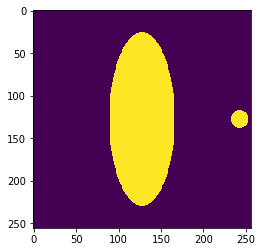
\includegraphics[width=\linewidth]{1_shape.png}
    \caption{给定介质的形状}
    \label{fig:1_data_plots:shape}
  \end{subfigure}%
  \hfill
  \begin{subfigure}[b]{0.3\textwidth}
    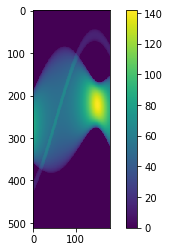
\includegraphics[width=\linewidth]{1_origin_data.png}
    \caption{原始扫描数据}
    \label{fig:1_data_plots:orig_data}
  \end{subfigure}%
  \hfill
  \begin{subfigure}[b]{0.2\textwidth}
    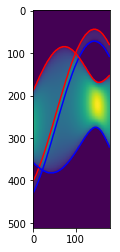
\includegraphics[width=\linewidth]{1_data_with_bounds.png}
    \caption{含边界的扫描数据}
    \label{fig:1_data_plots:orig_data_with_bounds}
  \end{subfigure}

  \caption{原始数据处理}
  \label{fig:1_data_plots} %% label for entire figure
\end{figure}

图\ref{fig:1_data_plots:shape}为题目给出的介质模板形状,我们以其中心(也是椭圆的中心)为原点建立笛卡尔坐标系$xoy$,对于此图$x$轴向右,$y$轴向上。同时我们以待求的探测系统的旋转中心为原点再建立笛卡尔坐标系$XOY$,$Y$轴正方向从接收器垂直指向探测器,$X$轴正方向指向接收器横坐标增大的方向。对于探测系统的接收器,坐标定义为:在数据第$i$行的接收器横坐标为$i - 255.5$;所有接收器纵坐标相等,规定为$-500$(只要探测器都在介质之外,其纵坐标大小不影响接受值)。

图\ref{fig:1_data_plots:orig_data}为根据题目给定的对模板的测量数据绘制的图,横轴为180个方向,纵轴为探测器编号,点颜色亮度表示吸收值。可知图中任意一条垂直线的宽度即为当前垂直X射线方向(即为平行探测器方向)的模型的宽度。图中有一条较明显的高度相同的正弦曲线形状的条带,容易推断为模板中圆形留下的图样;另一条宽度变化的条带,则为椭圆留下的图样。

首先进行较为粗略的数据提取,找到两条条带各自的边界(即,检测到吸收的接收器的范围)。方法思路为使用Python读取每一列数据,找到吸收值突变点。在两条带未重合的部分,识别十分简单。在重合部分,方法为从附近的未重合部分向上下进行试探,寻找最大值(观察可知图形上重合部分属于椭圆条带的边界比较亮)。图\ref{fig:1_data_plots:orig_data_with_bounds}为用此方法寻找到的两条带边界,基本与图形相吻合。但经过观察可知,条带图在峰、谷部分的边界并不明显(在数据上表现为各点值较接近,在图形上表现为边界线变“平”,边缘“黯淡”),这是由于接收器间具有一定的间隔造成的。故用这种方法得到的边界并不准确,无法直接用于后续计算。

\subsubsection{计算接收器间距与圆心位置}
\label{sec:1_calc_l}
\begin{figure}[htbp]
  \centering

  \begin{subfigure}[b]{0.48\textwidth}
    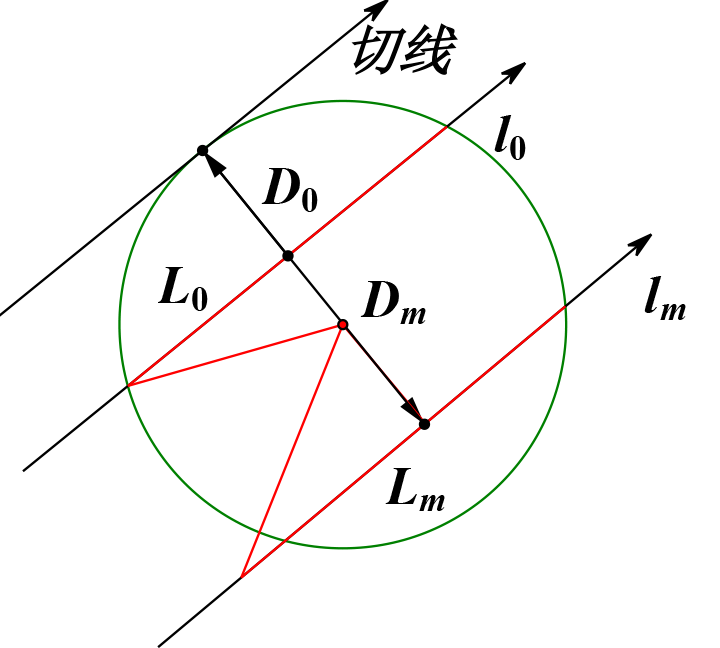
\includegraphics[width=\linewidth]{1_circle_lines.png}
    \caption{扫描线与圆的几何关系}
    \label{fig:1_circle_lines}
  \end{subfigure}%
  \hfill
  \begin{subfigure}[b]{0.48\textwidth}
    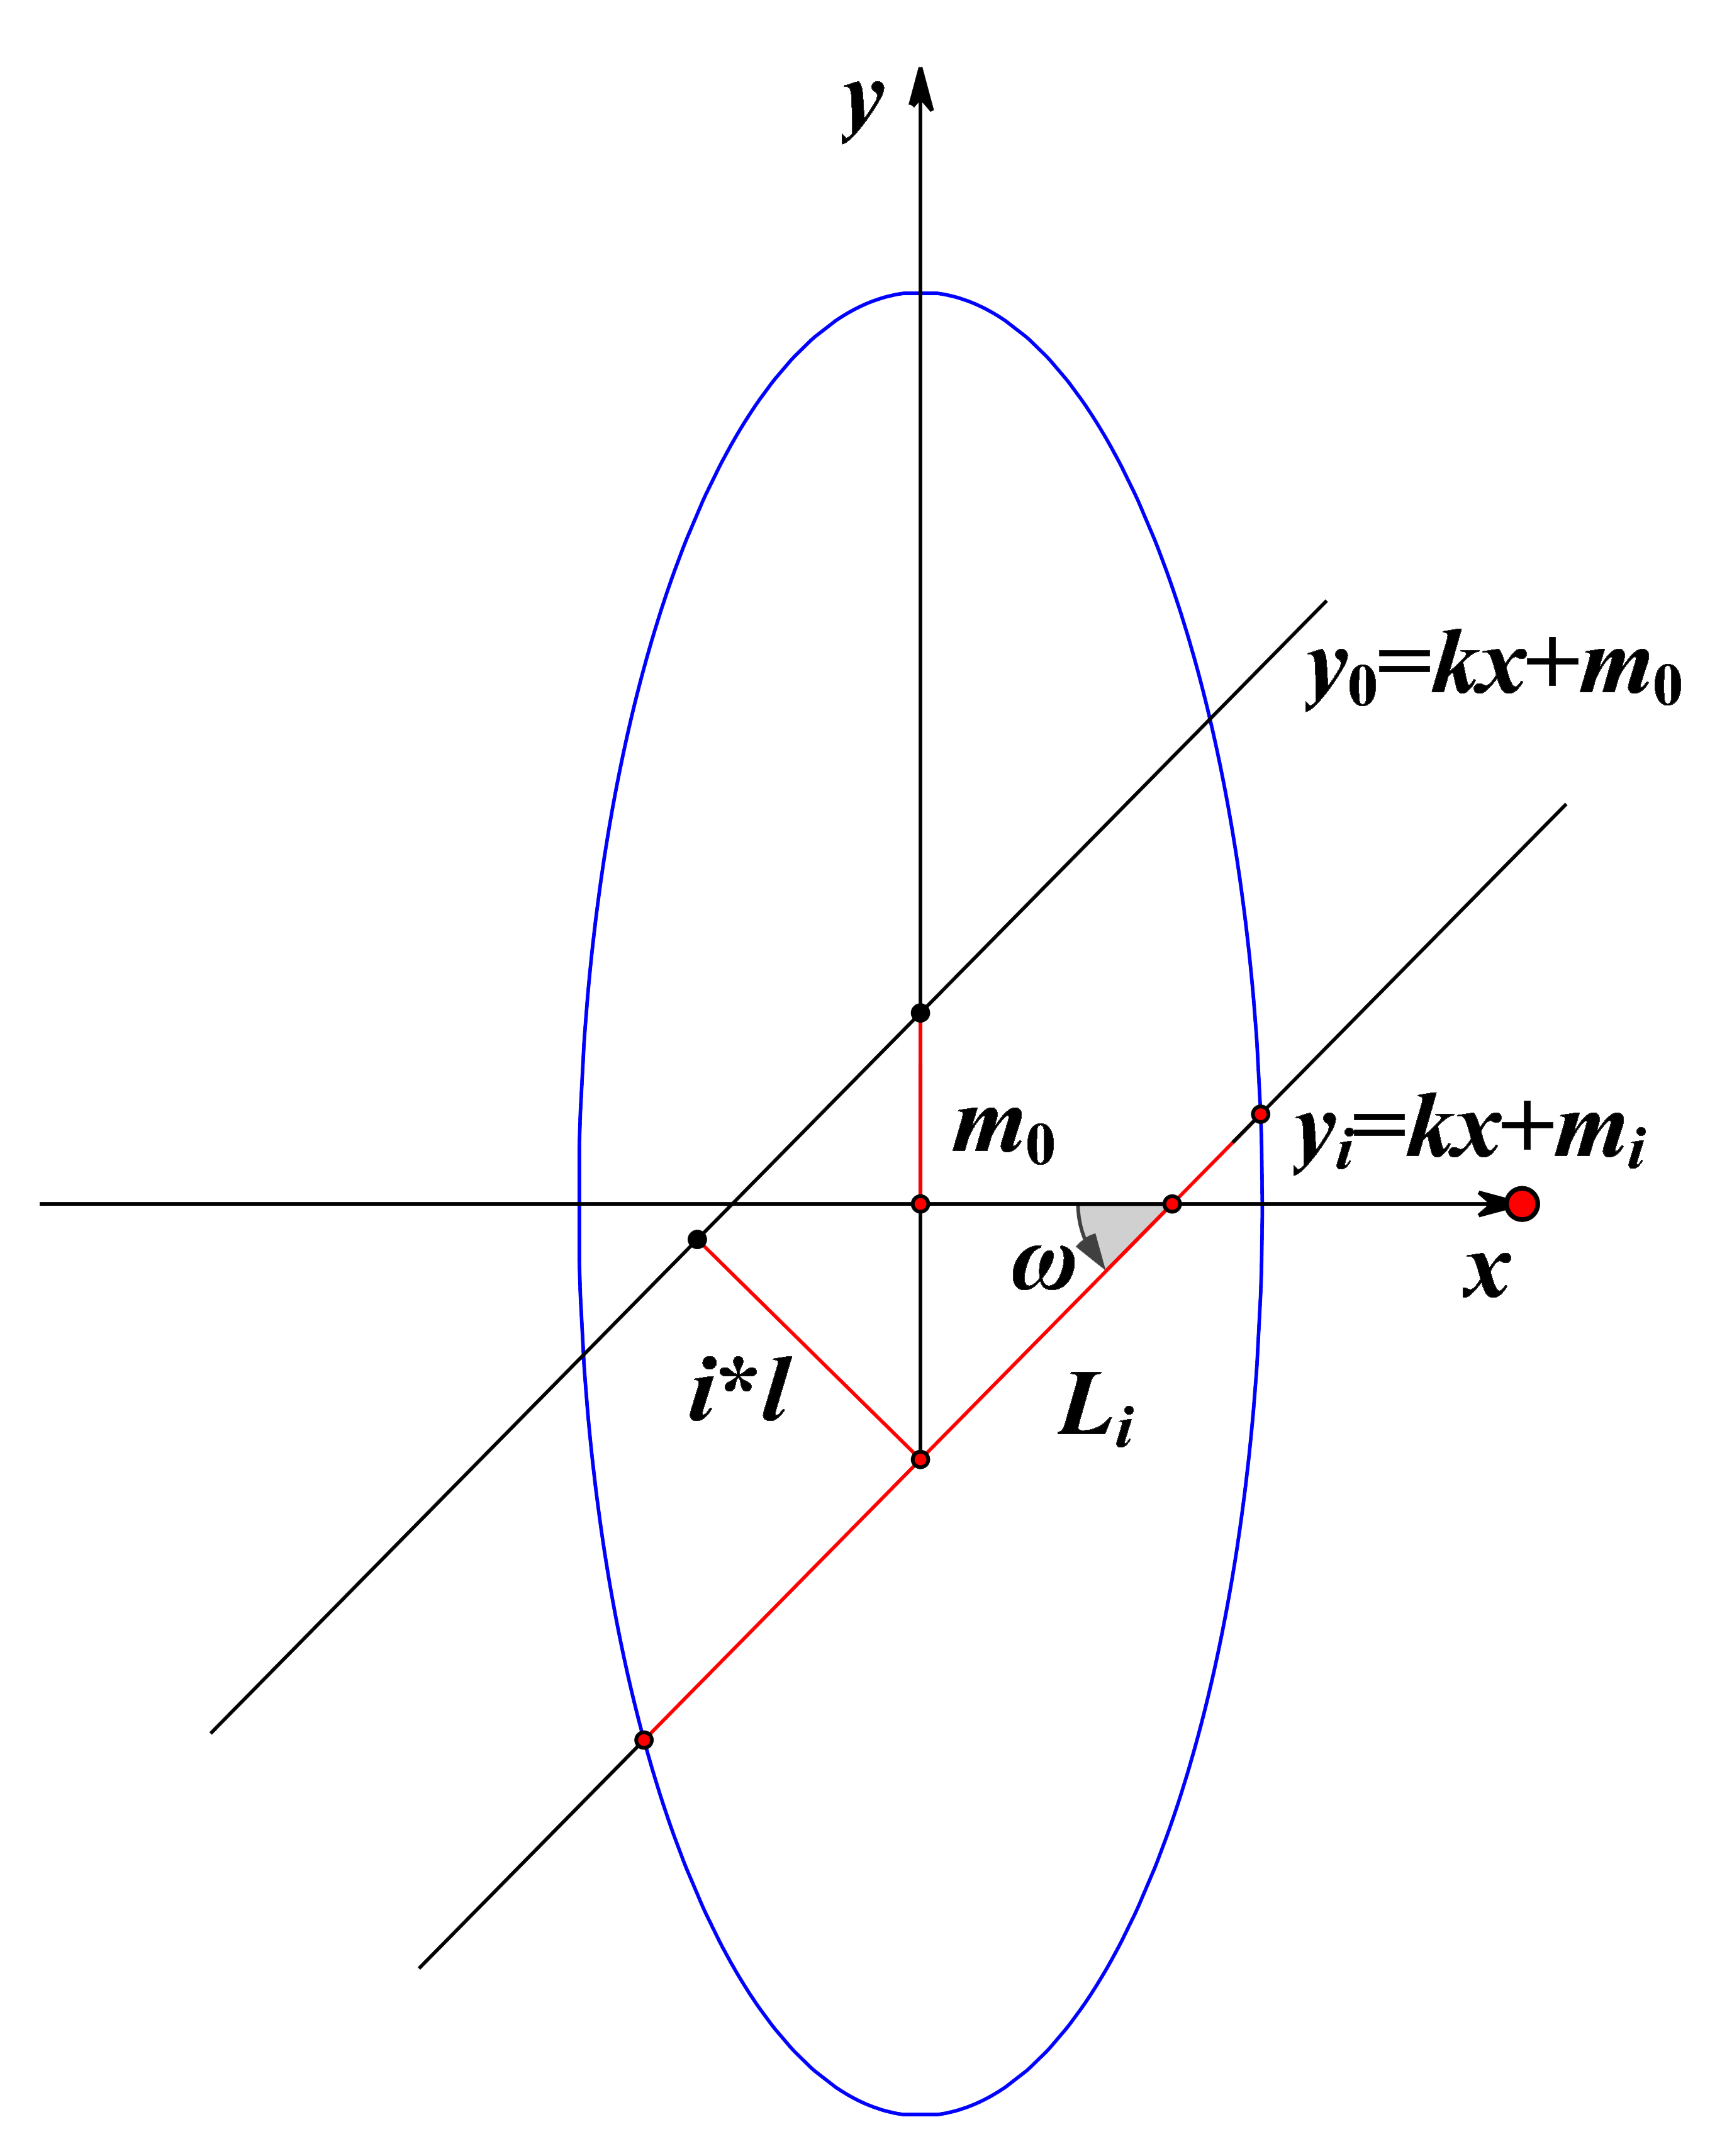
\includegraphics[width=\linewidth]{1_ellipse_lines.png}
    \caption{扫描线与椭圆的几何关系}
    \label{fig:1_ellipse_lines}
  \end{subfigure}%

  \caption{计算时几何关系的图示}
  \label{fig:1_geometry}
\end{figure}

考虑另一种思路,对于条带未重合时的数据,可精确地得知穿过圆的扫描线(即一个接收器接收到的信号)位置。下面的推导均在吸收值尺度下进行。考虑一个特定的方向,将这些线按接收器编号升序记为$l_0, l_1, \hdots, l_n$,共$n+1$条,对于第$m$条线定义“线长”即为对应接收器的读数$L_m$,定义“线距”$D_m$为第$m$条线与此方向下最靠近$l_0$的圆的切线之间的距离。根据图\ref{fig:1_circle_lines}中所描绘的几何关系,我们有
\begin{equation}\label{equ:1_circle}
  R^2=(D_m-R)^2+(\frac{L_m}{2})^2
\end{equation}
又由于$D_m=D_0+m l$,代入公式\ref{equ:1_circle}后与$m=0$时的情况相减,可得到
\begin{equation}\label{equ:1_reg}
  2 m l(D_0-R) + m^2 l^2 = \frac{L_0^2-L_m^2}{4}
\end{equation}
将$l(D_0-R)$与$l^2$作为未知系数,$2m$与$m^2$作为参数进行线性回归,可得到在这个方向下$l^2$的值。对所有条带未重合的方向重复该操作,取平均值,可得到$l_i=0.4903$(在SI制下$l=0.2766\,\si{mm}$)。这组数据的标准差为$\num{9.74e-4}$,稳定程度较高。

由于圆直径最长,而数据中属于圆的吸收值部分出现多次明显的最大值,故我们直接将每个旋转方向上吸收值最大值视为圆直径,再取这些值中的最大值后得$d_i=14.1796$。计算特定角度下圆心在旋转坐标系中的$X$坐标的方法也是简单的:在经过圆的所有扫描线中去掉线长$L_m$最大的两个$l_{max}, l_{max+1}$(一定相邻),则$l_0, l_1, \hdots, l_{max-1}$与$l_{max+2}, l_{max+3}, \hdots, l_n$分列圆心两侧,根据垂径定理(即公式\ref{equ:1_circle})即可计算出圆心与直线的距离,即可得到圆心的横坐标。对第$j$个旋转角度取得的所有坐标取均值,确定为该方向上圆心的横坐标$C_{x_j}$。当圆心横坐标确定后,我们根据横坐标与半径即可对于无重叠的部分圆条带重新确定一个更精确的边界,此边界的数值不再只落在接收器代表的点上。

\subsubsection{确定旋转角度与旋转中心}

由于探测系统所在的坐标系旋转时圆在其横轴上留下的投影位置发生变化,根据几何约束可求解旋转系统在每次投影时的旋转角度与其旋转中心相对模板的位置。具体推导如下(下列推导中,所有长度量的度量均以吸收量为尺度,略去尺度下标):

在$oxy$系中,考虑椭圆$x^2/a^2+y^2/b^2=1$(其中$a$、$b$分别为已知的两个半轴长)与扫描线$y=kx+m$,联立方程,根据解析几何知识容易知道直线截椭圆的弦长为:
\begin{equation}\label{equ:1_length}
  L = \sqrt{1+k^2}\sqrt{(x_1+x_2)^2-4 x_1 x_2} = \sqrt{k^2+1} \sqrt{\frac{4 a^4 k^2 m^2}{\left(a^2 k^2+b^2\right)^2}-\frac{4 a^2 \left(m^2-b^2\right)}{a^2 k^2+b^2}}
\end{equation}
将$XOY$系的两个轴正方向均与$oxy$系相同时的状态称为“初始位置”,当系统相对初始位置旋转角度为$\theta$时,扫描线与$ox$轴的夹角满足$\omega = \theta + \frac{\pi}{2}$。由于所有扫描线都是平行的,故第$i$条直线的截距$m_i$可以表示为$m_0+i\Delta m$,又由于$\Delta m = l / \cos(\pi-\omega) = -l/\cos\omega$,且$k=\tan\omega$。上述等式均可简单地由图\ref{fig:1_ellipse_lines}中表述的几何关系推导出。此时,方程\ref{equ:1_length}可约化为:
\begin{equation}\label{equ:1_degree_full}
  \sqrt{k^2+1} \sqrt{\frac{4 a^4 k^2 \left(i l \sqrt{k^2+1} +m_0\right){}^2}{\left(a^2 k^2+b^2\right)^2}-\frac{4 a^2 \left(\left(i l \sqrt{k^2+1} +m_0\right){}^2-b^2\right)}{a^2 k^2+b^2}}=L_i
\end{equation}

对于穿过椭圆的每一根直线,其$i$与$L_i$的值是确定的,于是方程\ref{equ:1_degree_full}便构成一个关于$k$与$m_0$的二元方程。在每一个方向上,都有足够多的扫描穿过椭圆(且不穿过圆),构成一个方程数量远多于未知数的超定方程组。我们将其相邻两两联立求解,舍去无用的$m_0$后将获得的$k$的绝对值(由于方程中均为关于$k$的偶次项,故一定会有正负两个根)进行平均,作为该方向上的扫描线斜率。在扫描线与$ox$轴接近垂直的角度上,三角函数会产生较大的误差,此时我们将直线方程重新设为$x=py+q$进行求解,求得的$|p|$为实际斜率绝对值的倒数。

在获得所有方向的$|k_i|$后,可据此计算出$\theta_i$的值;在一些临界值处的取值,是参考扫描数据的变化给出的。具体计算公式为:
\begin{equation}\label{equ:1_k_to_theta}
  \theta_i=
  \begin{cases}
    \frac{\pi}{2}-\arctan k_i, &  0 \leq i \leq 61 \\
    \frac{\pi}{2}+\arctan k_i, &  61 \leq i \leq 150 \\
    \frac{3\pi}{2}-\arctan k_i, & 151 \leq i \leq 179
  \end{cases}
\end{equation}
特别地,我们确定了第一组扫描数据对应的$\theta_0 = 0.51735\,\mathrm{rad} = 29.6420 \deg$

下一步确定旋转中心。初始位置中圆形的圆心在$XOY$系中坐标记为$C(X_0,Y_0)$,到$O$的距离$d=\sqrt{X_0^2+Y_0^2}$恒定。旋转中心在$oxy$系中的坐标即为$(-X_0,-Y_0)$。当$XOY$旋转$\theta$角度时,射线$OC$与$OX$轴形成有向角$\phi_\theta=\arg(X_0+iY_0)-\theta$(其中$i$为虚数单位),于是得到$C$的纵坐标$X_\theta=d\cos\phi_\theta$。由于在上面的过程中我们已经得到了部分旋转角度下比较精确的圆心坐标,将$\theta_i$与对应的$C_{x_i}$代入上面的推导即可获得关于$X_0$与$Y_0$的两个方程。由于数据较多,我们选取了两段未与椭圆重叠的圆条带(扫描序号分别为$0 \leq n \leq 13$与$110 \leq n \leq 180$),每次在两个集合中各选择一个扫描数据进行方程求解,共产生$910$组解。将其分别平均后得到的解为(在扫描线间距的尺度下)$X_{0\_s}= 196.0739, Y_{0\_s}= -22.6529$,转换尺度后易知探测系统的旋转中心在SI制下在$oxy$系中的坐标为$(-9.2383\,\si{mm}, 6.2663\,\si{mm})$,即位于模型板中心的略左上方位置处。